\documentclass[conference]{IEEEtran}
\IEEEoverridecommandlockouts
% The preceding line is only needed to identify funding in the first footnote. If that is unneeded, please comment it out.
\usepackage{cite}
\usepackage{amsmath,amssymb,amsfonts}
\usepackage[hidelinks]{hyperref}

\hypersetup{
    colorlinks=true,
    linkcolor=black,
    citecolor=black,
    urlcolor=black
}

\usepackage{algorithmic}
\usepackage{graphicx}
\usepackage{textcomp}
\usepackage{xcolor}
\usepackage{url}
\def\BibTeX{{\rm B\kern-.05em{\sc i\kern-.025em b}\kern-.08em
    T\kern-.1667em\lower.7ex\hbox{E}\kern-.125emX}}
\begin{document}

\title{Machine Unlearning for Object Detection Models: A Comparative Study\\
}

\author{\IEEEauthorblockN{Soumyadipta Kar}
\IEEEauthorblockA{\textit{University of Helsinki}, Finland \\
\url{https://orcid.org/0009-0008-1312-5538}}
}

\maketitle

\begin{abstract}
Machine unlearning is a critical technique for ensuring data privacy, regulatory compliance, and model trustworthiness in modern deep learning pipelines. While unlearning is widely studied in classification, its behavior in object detection and segmentation remains less explored in practical settings. In this work, we survey representative unlearning approaches and present an empirical case study on a YOLO segmentation model for microscopic leaf analysis. We evaluate four methods (Gradient Difference, SCRUB, SSD, and SISA-style unlearning) for class-level forgetting of trichome instances, and quantify the utility--forgetting--efficiency trade-off. On the test split, Gradient Difference, SCRUB, and SSD achieve complete forgetting for the target class (trichome mAP50 = 0.000), while SCRUB preserves the highest overall utility among these complete-forgetting methods (mAP50 = 0.454). SISA retains the strongest overall utility (mAP50 = 0.627) but only partially forgets trichome (mAP50 = 0.610). Energy tracking further shows SSD as the most energy-efficient method in our runs (0.00442 kWh).
\end{abstract}

\begin{IEEEkeywords}
machine unlearning, object detection, privacy
\end{IEEEkeywords}

\section{\textbf{Introduction}}
The rapid growth of machine learning models as an integral part of personalized applications, from facial recognition to content generation, has evidently led to increased user-privacy concerns and data-removal requests. Machine Learning as a Service (MLaaS) has only intensified this need, since such platforms operate on large volumes of potentially sensitive user data. As legal frameworks such as the General Data Protection Regulation (GDPR) in Europe and the California Consumer Privacy Act (CCPA) in the United States enforce the ``right to be forgotten,'' machine learning practitioners face a practical engineering challenge: how can we efficiently remove the influence of selected data points from a trained model without retraining everything from scratch? \cite{cao2015,bourtoule2021}

This challenge is particularly acute in computer vision systems where full retraining is expensive and the forgetting target can be semantically specific (e.g., one class in detection/segmentation). Therefore, beyond simple deletion guarantees, practical unlearning studies must jointly report: (i) forgetting efficacy, (ii) retain-set utility, and (iii) computational cost \cite{kurmanji2023,strubell2019}.

Our practical contributions are:
\begin{itemize}
    \item a reproducible object detection unlearning benchmark on the Birch stomata dataset;
    \item comparative evaluation of four implemented methods under the same base model and split protocol;
    \item joint reporting of mAP-based effectiveness and runtime/energy efficiency.
\end{itemize}

\section{\textbf{Motivation for Machine Unlearning}}

\subsection{Privacy and Legal Compliance}
Machine unlearning directly supports legal requirements such as user-requested data removal. In applied ML systems, deleting raw records is insufficient when model parameters still encode traces of that data \cite{cao2015,bourtoule2021}.

\subsection{Environmental Sustainability}
Frequent full retraining is energy intensive. Efficient unlearning methods can reduce compute and carbon footprint, especially when removal requests are recurrent \cite{strubell2019}.

\subsection{Operational Cost and Time Savings}
In production settings, model downtime and retraining costs are major bottlenecks. Practical unlearning methods target fast updates while preserving acceptable predictive quality.

\subsection{Model Maintenance and Concept Drift}
Unlearning can also support model maintenance by removing outdated or undesirable concepts while keeping useful knowledge intact.


\section{\textbf{Background}}

\subsection{Machine Unlearning} Let \(M\) denote a model trained on a dataset \(D\). We split \(D\) into two distinct subsets: the retain set \(D_r\), containing samples to be preserved, and the forget set \(D_f\), containing samples to be removed, such that \(D = D_r \cup D_f\) and \(D_r \cap D_f = \emptyset\)

The objective of machine unlearning is to obtain an updated model \(M'\) that behaves similarly to a model solely trained on \(D_r\), while avoiding the computational cost of retraining from scratch.

\subsection{Evaluation Metrics for Unlearning} Evaluating unlearning models is challenging because we need to balance two competing objectives: (1) effective removal of information associated with \(D_f\) and (2) preservation of performance on \(D_r\).

In this work we use class-wise and aggregate detection metrics:
\begin{itemize}
    \item \textbf{Test mAP50}: overall utility after unlearning;
    \item \textbf{Target-class (trichome) mAP50}: forgetting efficacy;
    \item \textbf{Runtime, energy, and CO\(_2\)}: operational efficiency.
\end{itemize}

Complete forgetting for the target class corresponds to target-class mAP50 approaching 0.


\section{\textbf{Unlearning Methods}}

This section contains both surveyed methods from the literature and the subset implemented in our benchmark.



\subsection{SISA Training (Exact Unlearning)}\label{AA}
SISA, which stands for Sharded, Isolated, Sliced, and Aggregated Training \cite{bourtoule2021}, is one of the oldest and most principled approaches  to unlearning. The idea of SISA is to split the training data into separate chunks called shards and train a separate sub-model on each one. When data needs to be removed, only the shard containing that data is retrained—not the whole model. This works best for models with smaller datasets because of the only downside—we have to save the checkpoints for each shard, which takes up quite a lot of storage. 

\subsection{Gradient Ascent (GA)}
Gradient Ascent \cite{graves2021} is one of the simplest unlearning methods. In a normal training setup, we usually minimize the loss function on the training data. what gradient Ascent does is the opposite for the forget set: it maximizes the loss, pushing the model to make worse predictions on \(D_f\). Formally, the update is:
\begin{equation}
\theta' = \eta \nabla_\theta L(M_\theta, D_f)\label{eq}
\end{equation}
In practice, this is alternated with normal training steps on \(D_r\) to make sure that  the model does not suffer catastrophic degradation.


\subsection{Fine-tuning on Retain Set (FT)}
Finetuning on the retrain set is a straightforward baseline involving continuous training of the model exclusively on \(D_r\) after the forget set has been removed.

\subsection{ERM-based Unlearning}
ERM-based unlearning \cite{chundawat2023} combines two objectives at once: minimize loss on the retain set (standard training) and maximize loss on the forget set (Gradient Ascent), balanced by a tunable parameter \(\lambda\).



\subsection{SCRUB}\label{SCM}
SCRUB (Selective Categorical Removal via Unlearning Backpropagation) \cite{kurmanji2023} introduces a teacher-student framework for unlearning. The original model \(M\) acts as the teacher, and the unlearned model \(M'\) is the student. The student learns to match the teacher's behavior on \(D_r\) using knowledge distillation, while simultaneously using Gradient Ascent on \(D_f\). This distillation step helps \(M'\) retain a deep understanding of the retain data, not just its final predictions. This makes SCRUB more stable and better preserving model quality than plain Gradient Ascent. 

\subsection{Influence Function}
Influence-function-based methods estimate how individual training points affect predictions and can be used to approximate removal without retraining \cite{koh2017}. We discuss them for completeness; they are not implemented in our experiments.

\subsection{SALUN (Saliency-Based Unlearning)}
SALUN selectively updates high-saliency parameters to efficiently remove forget-set information while minimizing utility collapse \cite{fan2024}. We discuss SALUN in the survey context; the current empirical benchmark focuses on Gradient Difference, SCRUB, SSD, and SISA-style unlearning.

\subsection{Implemented Methods in This Benchmark}
The empirical benchmark in this paper reports results for four implemented methods: Gradient Difference, SCRUB, SSD, and SISA-style unlearning. Methods such as SALUN, influence-function variants, and diffusion-model unlearning are surveyed but not executed in this project.

\section{Experimental Setup}
\subsection{Hardware and Software}
All experiments are run on an Apple Silicon MacBook (MPS backend enabled) using Python and Ultralytics YOLO segmentation tooling. We use one fixed baseline checkpoint and a shared orchestration pipeline so that each unlearning method starts from the same initialization and data split.

\subsection{The Birch Stomata Dataset}
The dataset contains four categories: \textit{nothing}, \textit{stomata}, \textit{trichome}, and \textit{vein}. We perform class-level unlearning for \textit{trichome}. In annotation-mode splitting, trichome annotations are removed from the retain data while other annotations are preserved.

Observed split statistics are:
\begin{itemize}
    \item train: 899 images, 46,979 annotations;
    \item validation: 51 images, 2,750 annotations;
    \item test: 49 images, 2,569 annotations.
\end{itemize}

\subsection{Experimental Protocol}
We start from the same baseline model \(M_0\) for all methods. We evaluate Gradient Difference, SCRUB, SSD, and SISA-style unlearning. Performance is measured on validation and test splits with consistent metric extraction. Baseline test mAP50 is 0.6773 and baseline trichome mAP50 is 0.7284.

\begin{table}[htbp]
\caption{Main Test-Set Unlearning Results}
\begin{center}
\begin{tabular}{|l|c|c|c|}
\hline
\textbf{Method} & \textbf{Test mAP50} & \textbf{Trichome mAP50} & \textbf{Forgetting} \\
\hline
Baseline & 0.6773 & 0.7284 & None \\
\hline
Gradient Difference & 0.3754 & 0.0000 & Complete \\
\hline
SCRUB & 0.4537 & 0.0000 & Complete \\
\hline
SSD & 0.3971 & 0.0000 & Complete \\
\hline
SISA & 0.6270 & 0.6104 & Partial \\
\hline
\end{tabular}
\label{tab1}
\end{center}
\end{table}

\begin{figure}[htbp]
\centerline{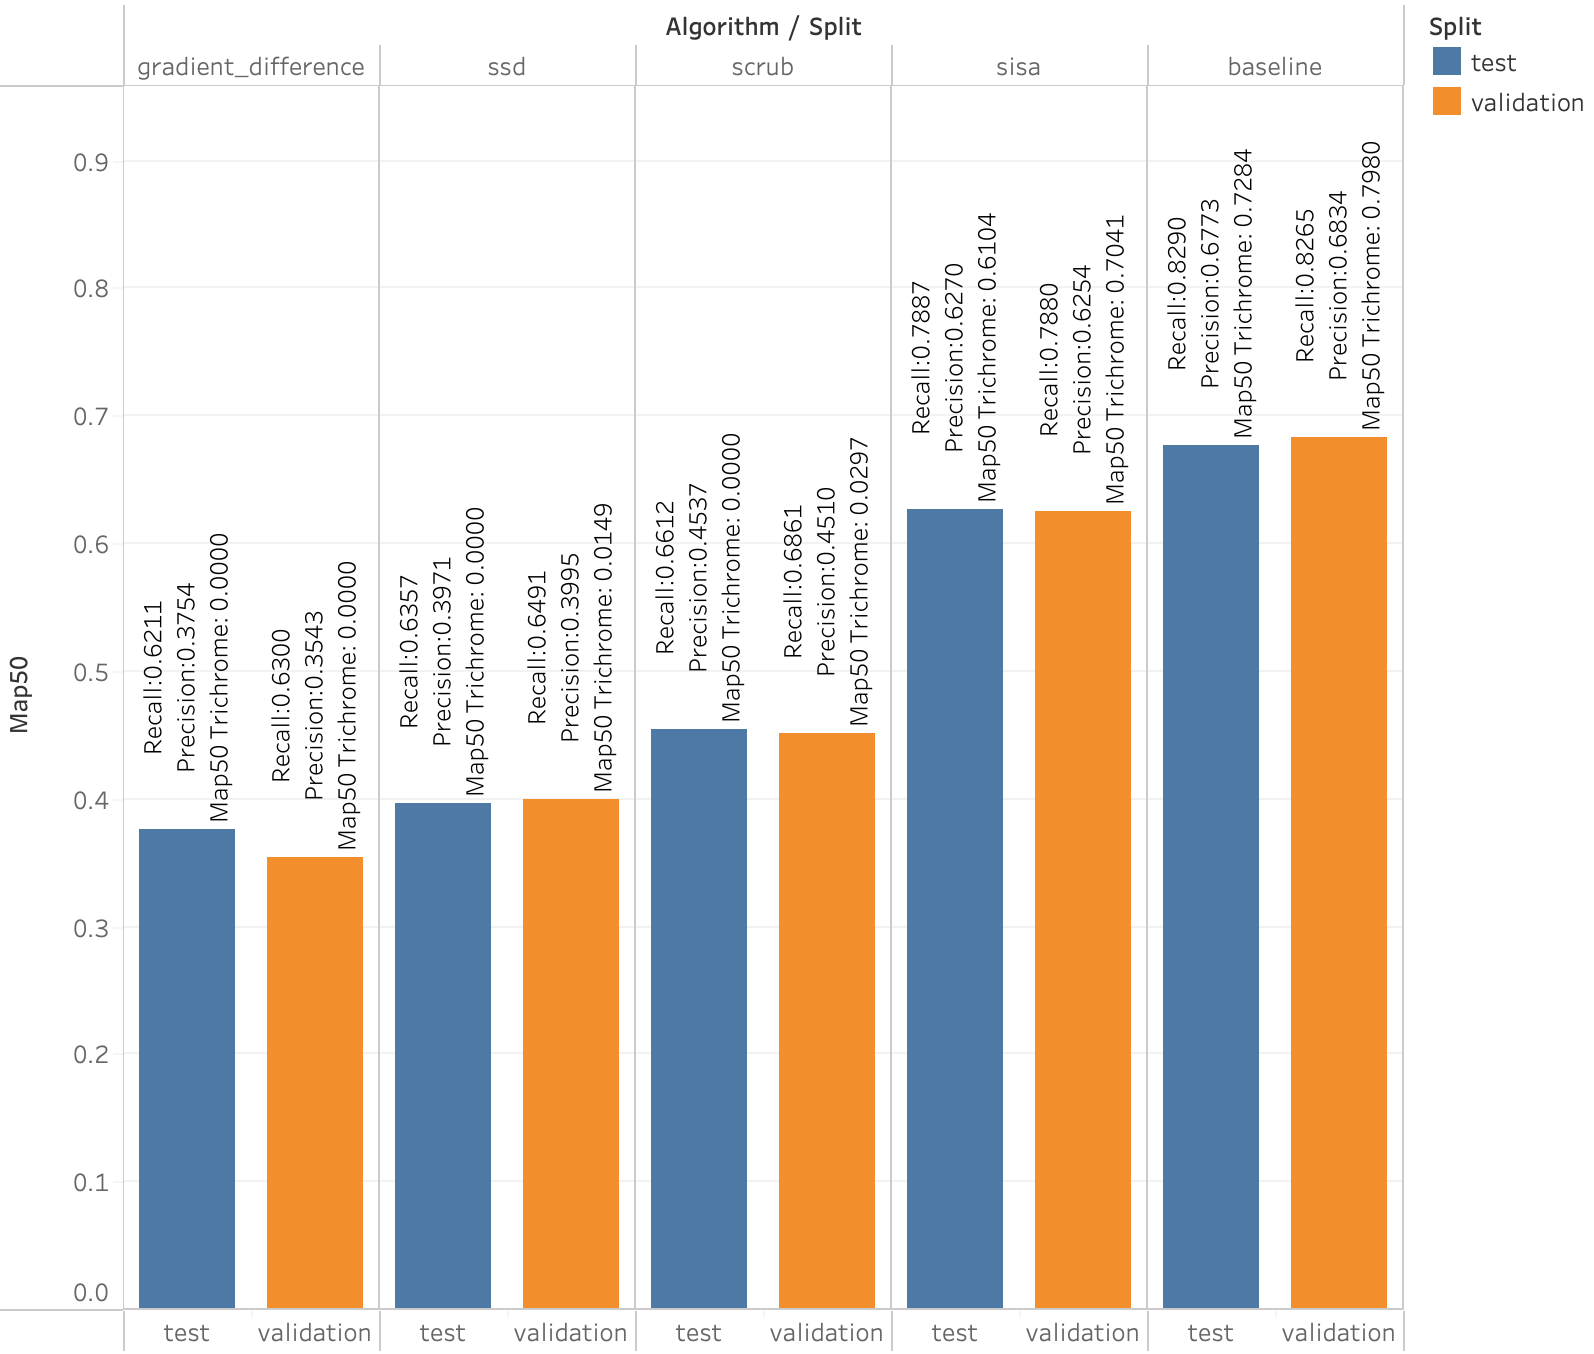
\includegraphics[width=0.48\textwidth]{results_figures/model_comparison_metrics.png}}
\caption{Overall utility comparison (mAP50) across algorithms and splits, with precision/recall labels for context.}
\label{fig:model_comparison}
\end{figure}

\begin{table}[htbp]
\caption{Efficiency Comparison (Annotation Benchmark)}
\begin{center}
\begin{tabular}{|l|c|c|c|}
\hline
\textbf{Method} & \textbf{Runtime (s)} & \textbf{Energy (kWh)} & \textbf{CO\(_2\) (kg)} \\
\hline
Gradient Difference & 1319.0 & 0.01282 & 0.00513 \\
\hline
SCRUB & 1039.2 & 0.00794 & 0.00318 \\
\hline
SSD & 1949.8 & 0.00442 & 0.00177 \\
\hline
SISA & 4569.1 & 0.02217 & 0.00887 \\
\hline
Retain-only retraining & 1229.1 & 0.01195 & 0.00478 \\
\hline
\end{tabular}
\label{tab2}
\end{center}
\end{table}

\begin{figure}[htbp]
\centerline{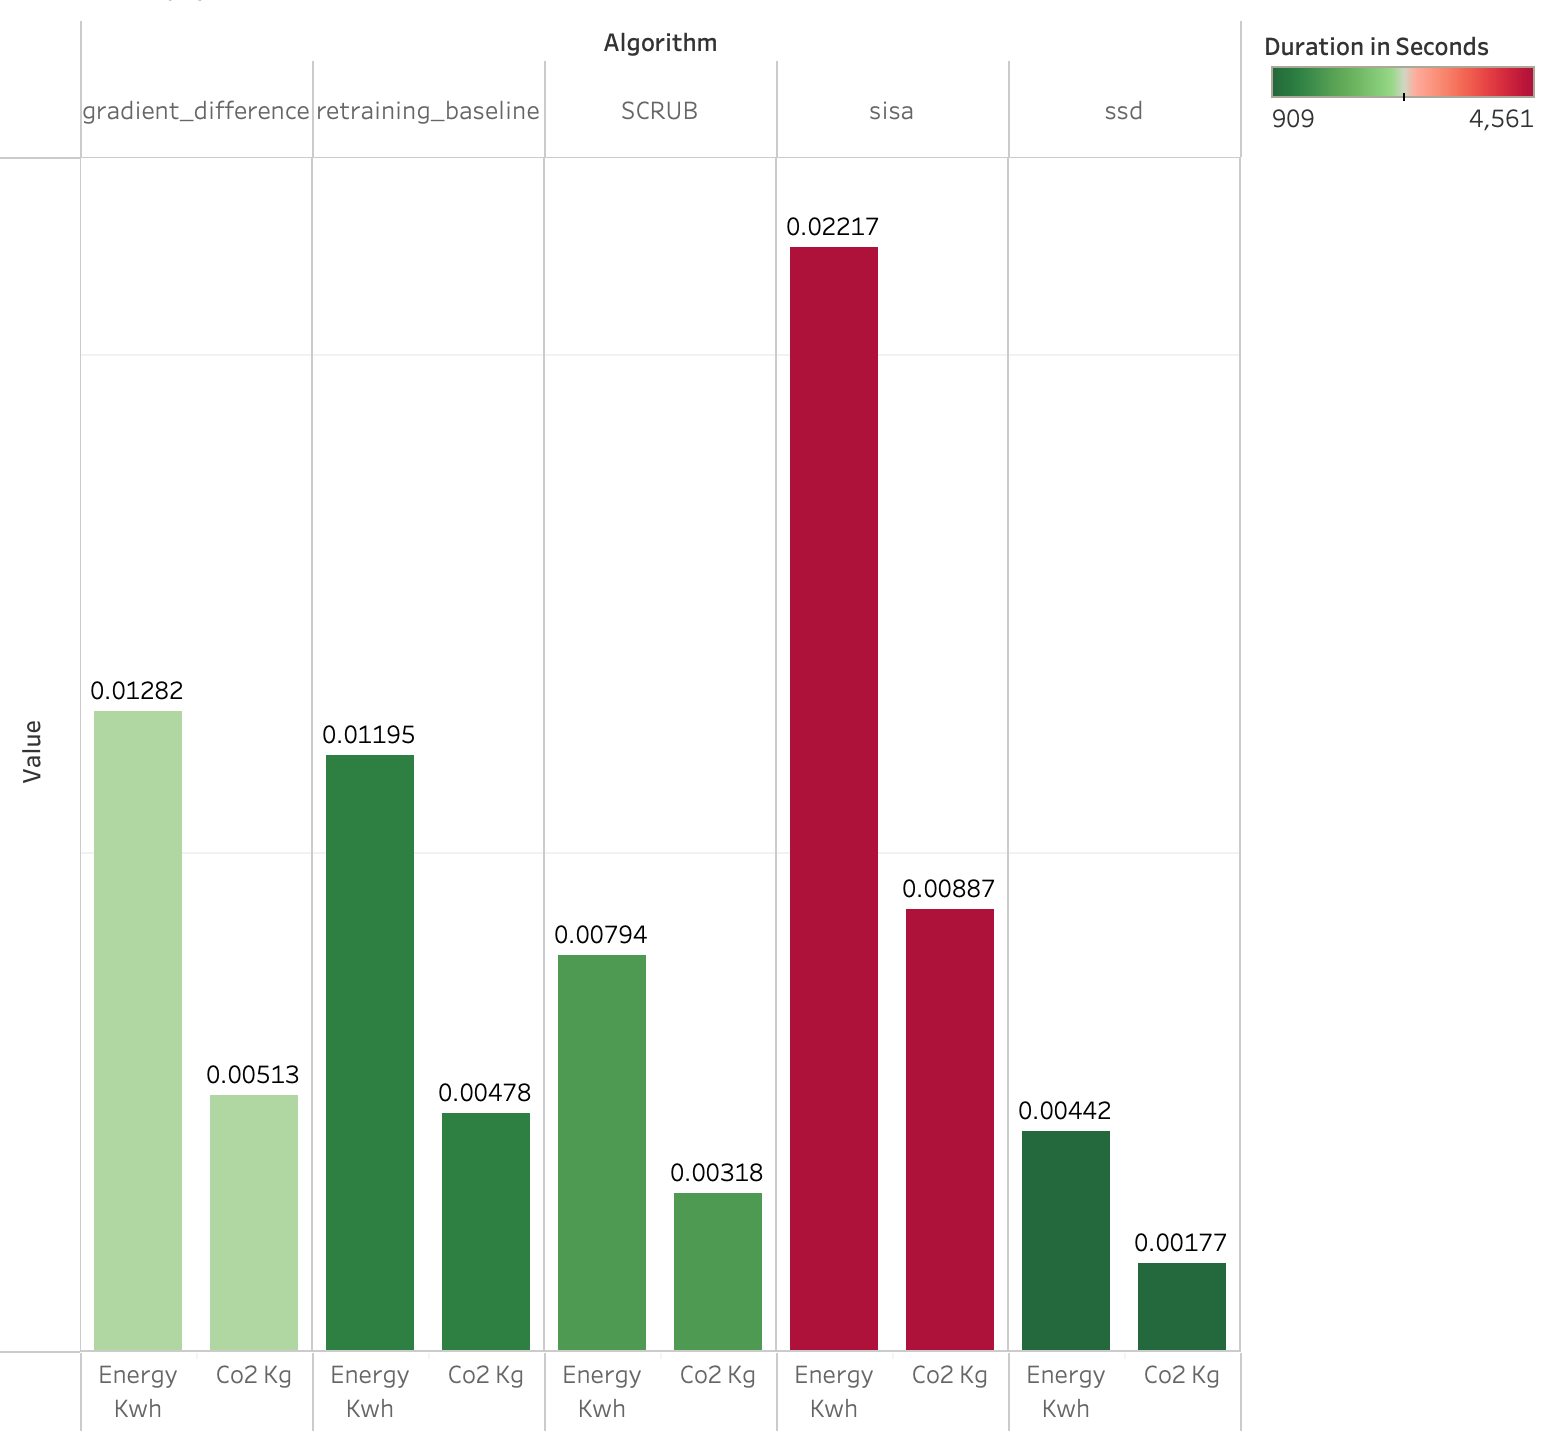
\includegraphics[width=0.48\textwidth]{results_figures/energy_comparison_annotation.png}}
\caption{Energy (kWh) and CO\(_2\) (kg) comparison across methods; bar color encodes duration in seconds.}
\label{fig:energy_comparison}
\end{figure}

\section{Results and Analysis}
From Table~\ref{tab1} and Figure~\ref{fig:model_comparison}, the baseline remains strongest in overall utility (test mAP50 = 0.6773), while unlearning introduces a predictable utility drop. Among strict-forgetting methods, SCRUB gives the best balance (test mAP50 = 0.4537), followed by SSD (0.3971) and Gradient Difference (0.3754).

The class-wise view in Figure~\ref{fig:scrub_classwise} helps interpret this behavior. For SCRUB, trichome is fully forgotten on test (mAP50 = 0.0000) but retains a very small residual on validation (mAP50 = 0.0297). At the same time, the model still preserves high utility on stomata (test: 0.9350, validation: 0.9427), while ``nothing'' and ``vein'' classes show moderate degradation compared with baseline.

SISA follows a different trade-off: it retains high global utility (test mAP50 = 0.6270, closest to baseline) but does not satisfy strict target-class forgetting (trichome test mAP50 = 0.6104). This confirms that high retention quality does not automatically imply strong deletion quality.

Efficiency trends in Table~\ref{tab2} and Figure~\ref{fig:energy_comparison} are also clear. SSD is the lowest-energy method (0.00442 kWh, 0.00177 kg CO\(_2\)), SCRUB is next (0.00794 kWh, 0.00318 kg CO\(_2\)), while SISA is the most expensive (0.02217 kWh, 0.00887 kg CO\(_2\)). The retain-only retraining baseline sits between these extremes and remains more expensive than SSD and SCRUB.

\begin{figure}[htbp]
\centerline{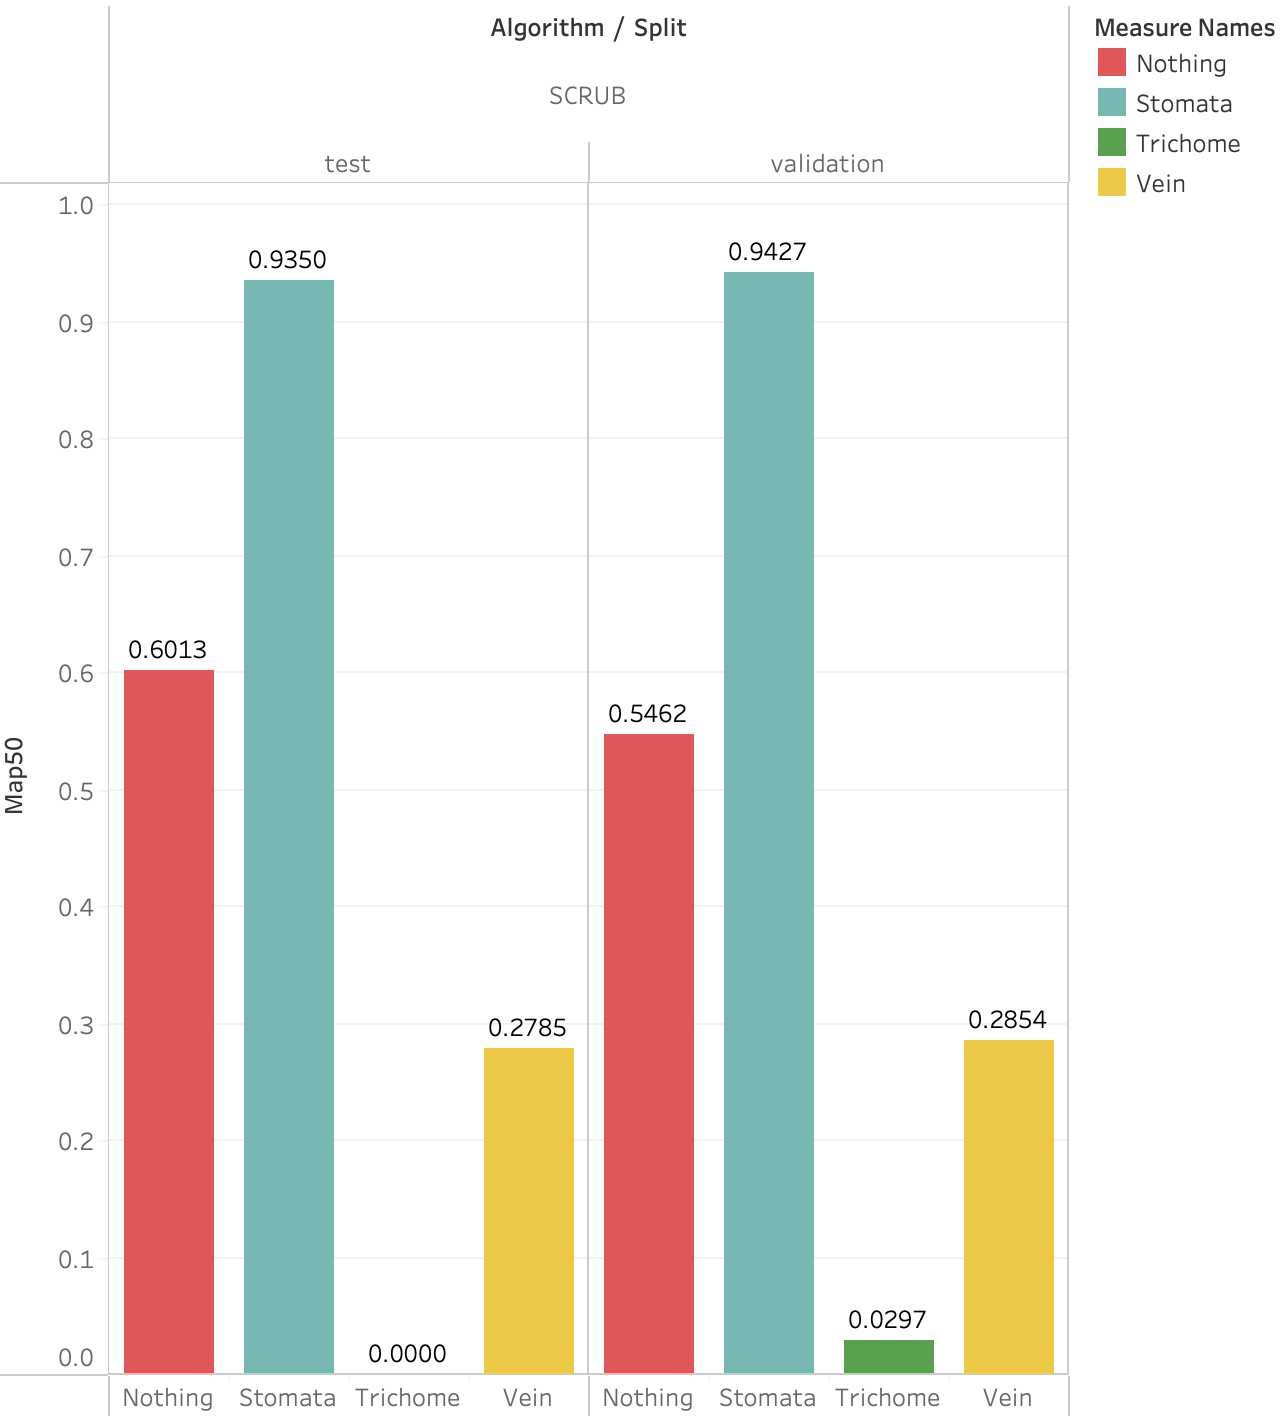
\includegraphics[width=0.48\textwidth]{results_figures/scrub_classwise_map50_valid_vs_test.png}}
\caption{SCRUB per-class mAP50 on validation and test splits; trichome suppression is strongest on test.}
\label{fig:scrub_classwise}
\end{figure}

\section{Discussion}
The updated plots reinforce one practical message: evaluation must be multi-objective. Looking only at global mAP50 would favor SISA, while looking only at forgetting would favor methods such as SCRUB/SSD/Gradient Difference. In practice, deployment requirements decide which objective dominates.

For strict deletion policies, SCRUB and SSD are safer choices in this benchmark, with SCRUB offering better utility and SSD offering better energy efficiency. For scenarios where utility preservation dominates and deletion tolerance is looser, SISA remains attractive.

The study still has limitations. Energy and CO\(_2\) values are estimate-backend values under fixed watt assumptions, so they should be interpreted as comparative indicators rather than absolute carbon accounting. Experiments are also limited to one dataset and one hardware environment. Finally, some surveyed methods (e.g., SALUN and diffusion-specific methods) are not implemented in this benchmark and remain future work.

\section*{Conclusion}
This paper presents a practical benchmark of machine unlearning for YOLO-based microscopic object detection. Using the updated evaluation plots, we confirm that complete test-set class forgetting is achievable (Gradient Difference, SCRUB, SSD), but always with some utility trade-off versus the baseline model. Among strict-forgetting methods, SCRUB provides the strongest utility retention, while SSD is the most energy- and CO\(_2\)-efficient. SISA remains the strongest in overall utility but does not achieve strict forgetting of the target class. Overall, the results support treating machine unlearning as a multi-objective engineering problem that jointly optimizes deletion quality, retained performance, and computational efficiency.



\begin{thebibliography}{16}

\bibitem{cao2015}
Y. Cao and J. Yang, “Towards making systems forget with machine unlearning,” in \textit{Proc. IEEE Symp. Security and Privacy (S\&P)}, 2015.

\bibitem{shokri2017}
R. Shokri, M. Stronati, C. Song, and V. Shmatikov, “Membership inference attacks against machine learning models,” in \textit{Proc. IEEE Symp. Security and Privacy (S\&P)}, 2017.

\bibitem{fredrikson2015}
M. Fredrikson, S. Jha, and T. Ristenpart, “Model inversion attacks that exploit confidence information and basic countermeasures,” in \textit{Proc. ACM Conf. Computer and Communications Security (CCS)}, 2015.

\bibitem{carlini2023}
N. Carlini, F. Tramer, E. Wallace, M. Jagielski, A. Herbert-Voss, K. Lee, A. Roberts, T. Brown, D. Song, U. Erlingsson, A. Oprea, and C. Raffel, “Extracting training data from diffusion models,” in \textit{Proc. USENIX Security Symp.}, 2023.

\bibitem{strubell2019}
E. Strubell, A. Ganesh, and A. McCallum, “Energy and policy considerations for deep learning in NLP,” in \textit{Proc. Annu. Meeting Assoc. Comput. Linguistics (ACL)}, 2019.

\bibitem{kumari2023}
N. Kumari, B. Zhang, R. Zhang, and J.-Y. Zhu, “Ablating concepts in text-to-image diffusion models,” in \textit{Proc. IEEE Int. Conf. Computer Vision (ICCV)}, 2023.

\bibitem{gandikota2023}
D. Gandikota, Y. Orgad, and B. Feizi, “Erasing concepts from diffusion models,” in \textit{Proc. IEEE Int. Conf. Computer Vision (ICCV)}, 2023.

\bibitem{bourtoule2021}
L. Bourtoule, V. Chandrasekaran, P. Choquette-Choo, H. Jia, A. Travers, B. Zhang, D. Lie, and N. Papernot, “Machine unlearning,” in \textit{Proc. IEEE Symp. Security and Privacy (S\&P)}, 2021.

\bibitem{graves2021}
A. Graves, V. Gandikota, and B. Feizi, “Amnesiac machine learning,” in \textit{Proc. AAAI Conf. Artificial Intelligence}, 2021.

\bibitem{chundawat2023}
J. Chundawat, A. Tarun, M. Mandal, and M. Kankanhalli, “Zero-shot machine unlearning,” \textit{IEEE Trans. Inf. Forensics Security}, 2023.

\bibitem{kurmanji2023}
A. Kurmanji, P. Triantafillou, J. Hayes, and E. Triantafillou, “Towards unbounded machine unlearning,” in \textit{Proc. Adv. Neural Inf. Process. Syst. (NeurIPS)}, 2023.

\bibitem{koh2017}
P. W. Koh and P. Liang, “Understanding black-box predictions via influence functions,” in \textit{Proc. Int. Conf. Machine Learning (ICML)}, 2017.

\bibitem{agarwal2017}
A. Agarwal, O. Dekel, and L. Xiao, “Second-order stochastic optimization for machine learning in linear time,” \textit{J. Mach. Learn. Res.}, vol. 18, 2017.

\bibitem{fan2024}
J. Fan, Y. Liu, Q. Chen, and Z. Wang, “Salun: Empowering machine unlearning via gradient-based weight saliency in both image classification and generation,” in \textit{Proc. Int. Conf. Learning Representations (ICLR)}, 2024.

\bibitem{di2021}
Z. Di, Z. Tian, J. He, and D. Tao, “Hidden killer: Invisible textual backdoor attacks with syntactic trigger,” arXiv preprint arXiv:2105.12400, 2021.

\bibitem{shumailov2023}
T. Shumailov, Z. Shumaylov, Y. Zhao, N. Papernot, R. Anderson, and Y. Gal, “Forget unlearning: Towards true data-deletion in machine learning,” in \textit{Proc. Int. Conf. Machine Learning (ICML)}, 2023.

\end{thebibliography}

\end{document}
